\documentclass{article}

\usepackage[margin=0.2cm]{geometry}
\usepackage{amsmath}
\usepackage{amssymb}
\usepackage{ulem}
\usepackage{hyperref}
\usepackage{minted}
\usepackage{multicol}
\usepackage{graphicx}
\usepackage{float}
\usepackage{subfigure}


\begin{document}

\tableofcontents

\newpage
\section{Hall's marriage theorem}
Let $G=(V,E)=(X+Y,E)$ be a bipartite graph, $G$ has a complete matching from $X$ to $Y$ iff $\forall S\subseteq X\ |S|\leq |N(S)|$,\\
where $N_G(S)=\{y\in Y\mid \exists x\in S\ (x,y)\in E\}$.



\subsubsection{sufficiency}
($\Rightarrow$)\quad
Let $M=\{(x,f(x))\in E\mid x\in X\}\subseteq E$ be a complete matching.\\
$N_G(S)=\{y\in Y\mid \exists x\in S\ (x,y)\in E\}\supseteq \{f(x)\mid x\in S\}$.

\subsubsection{necessity}
($\Leftarrow$)\quad
Apply induction on $|X|$.
\begin{enumerate}
	\item When $|X|=1$, the necessity is hold.
	\item Suppose that the necessity is hold, for $|X|\leq k$
	\item For $|X|=k+1$, $\forall S\subseteq X\ |S|\leq |N_G(X)|$
	      \begin{itemize}
		      \item $\forall \varnothing\subsetneq S\subsetneq X\ |N_G(S)|>|S|$\\
		            Select any edge $e=(x,y)$. Remove the vertices $x,y$ and every edges $(u,v)$ to get $G'$ s.t. $x\in\{u,v\}\lor y\in\{u,v\}$.\\
		            In $G'$, $\forall \varnothing\subsetneq S\subseteq (X\setminus \{x\})\quad |N_{G'}(S)|\geq |N_{G}(S)|-1\geq |S|$.\\
		            So we can find a complete matching  $M':X'\to Y'$ in $G'$.\\
		            Thus A complete matching $M:X\to Y$ can generated by $M'\cup \{(x,y)\}$
		      \item $\exists \varnothing\subsetneq S\subsetneq X\ |N_G(S)|=|S|$\\
		            Let $G_0=(V_0,E_0),G_1=(V_1,E_1)$ be two induced subgraph of $G$, where $V_0=S+N_G(S),V_1=(X\setminus S)+ (Y\setminus N_G(S))$.
		            \begin{itemize}
			            \item For $G_0$: $\forall P\subseteq S\ N_{G_0}(P)=N_{G}(P)$ so $\forall P\subseteq S\ |N_{G_0}(P)|=|N_{G}(P)|\geq |P|$.
			            \item For $G_1$: We claim that $\forall Q\subseteq (X\setminus S)\ |N_{G_1}(Q)|\geq |Q|$.\\
			                  Otherwise, let $Q_0$ be a subset s.t. $|N_{G_1}(Q_0)|<|Q_0|$.\\
			                  Then $N_{G}(S\cup Q_0)=N_{G}(S)\cup N_{G}(Q_0)$, where $N_{G}(S)=N_{G_0}(S),\ N_{G}(Q_0)\subseteq (N_{G}(S)\cup N_{G_1}(Q)),\ N_{G_1(Q_0)}\cap N_G(S)=\varnothing$.\\
			                  which leads to $|N_{G}(S\cup Q_0)|=|\leq |N_G(S)|+|N_{G_0}(Q_0)| < |S|+|Q_0|$, however $|N_{G}(S\cup Q_0)|\geq |S\cup Q_0|=|S|+|Q_0|$.\\
			                  Therefore in $G_1$, $\forall Q\subseteq (X\setminus S)\ |N_{G_1}(Q)|\geq |Q|$.\\
		            \end{itemize}
		            We can find a complete matching by merging the complete matching in $G_0$ and $G_1$.
	      \end{itemize}
\end{enumerate}

\subsubsection{generalization}

In a bipartite graph $G=(X+Y,E)$
Let $\mathrm{def}_G(S)=|S|-|N_G(S)|$,
then the size of maximum matching in $G$ is $|X|-\max_{\varnothing\subseteq S\subseteq X}\mathrm{def}_G(S)$

\newpage
\section{Havel-Hakimi algorithm}

\subsubsection{the theorem}

Given a list of non-negative integers $(d_1,d_2\ldots d_n)$ where $d_1\geq d_2\geq d_3\ldots d_n\geq 0$.\\
Is there a undirected simple\footnote{no loops $(v,v)$, no dup-edges $k\times (v,v)$} graph $G=(V,E)$ s.t. the degree sequence of $G$ is $(d_1,d_2\ldots d_n)$?

\begin{minted}{python}
from typing import List
def check(deg_seq: List[int]) -> bool:
    if len(deg_seq)==0:
        return True

    head,seq = deg_seq[0],deg_seq[1:]
    if len(seq)>=head:
        for i in range(head):
            seq[i]=seq[i]-1
        seq = sorted(seq, reverse=True)
        return seq[-1]>=0 and check(seq)
    return False
\end{minted}

\subsubsection{proof}

\emph{TODO}



\newpage
\section{graph isomorphism invariant}

\subsection{degree sequence}

$G\cong H\implies f(G)=H(G)$, where $f(G)=\mathrm{multi-set}\{\deg_G(v)\mid v\in G\}$.\\
This is a necessary but not sufficient condition, see the following example, where $H,G$ have the same degree sequence but are not isomorphic to each other.

\begin{minted}{C}
//!/usr/bin/dot
// in graphviz dot
graph G{
	1 -- 2
	2 -- 3
	3 -- 4
	4 -- 5
	2 -- x
}
graph H{
	1 -- 2
	2 -- 3
	3 -- 4
	4 -- 5
	3 -- x
}
\end{minted}


\newpage
\section{Lower bound of $\max(\omega(G),\alpha(G))$}

\subsection{futher readings}
\href{https://en.wikipedia.org/wiki/Ramsey_theory}{wikipedia: Ramsey theory}

\subsection{statement}

(Ramsey's Theorem) Every graph with $n$ vertices contains either a clique or an independent set with at least $\frac{1}{2}\log_2 n$ vertices.\\
$\omega(G)$: the clique number.
$\alpha(G)$: the independence number.

\subsection{proof}

\begin{enumerate}
	\item $n=1$, hold
	\item $n=2$, hold
	\item Suppose that $n=1,2,3\ldots k$, the statement is true\\
	      For $n=k+1$, select a arbitary vertex $u$.
	      Let $A=\{v\mid \{u,v\}\in E,v\neq u\},\, B=\{v\mid \{u,v\}\not\in E,v\neq u\}$
	      \begin{itemize}
		      \item $A$, there exists a clique $C$ of at least $\frac{1}{2}\log_2 |A|$ vertices.
		            $C+\{u\}$ is still a clique.
		      \item $B$, there exists a independent set $I$ of at least $\frac{1}{2}\log_2 |B|$ vertices.
		            $I+\{u\}$ is still an independent set.
	      \end{itemize}
	      Therefore, we can find either a clique or an independent set consisting of at least $1+\frac{1}{2}\max\left(\log_2 |A|+\log_2 |B|\right)$\\
	      $|A+B|=|A|+|B|=n-1=k\implies \max(|A|,|B|)\geq \frac{1}{2}k\implies \max\left(\log_2 |A|,\log_2 |B|\right)\geq -1+\log_2 k$\\
	      Thus $\max(\omega(G),\alpha(G))\geq 1+\left(-1+\log_2 k\right)=\log_2 k\geq \frac{1}{2}\log_2 n$
\end{enumerate}


\newpage
\section{Sufficient conditions for existence of a hamilton circuit }

\begin{itemize}
	\item Dirac's Theorem:
	      A simple graph $G=(V,E)$ s.t. $|V|\geq 3$ and $\forall v\in V\ \deg(v)\geq \frac{|V|}{2}$ has a Hamilton circuit.
	\item Ore's Theorem:
	      A simple graph $G=(V,E)$ s.t. $|V|\geq 3$ and $\forall \{u,v\}\left( \{u,v\}\not\in E\rightarrow \deg(u)+\deg(v)\geq |V|\right)$
\end{itemize}

\subsection{proof}

\newpage
\section{Kuratowski's Theorem: the equivalent condition of planar graph}


\subsection{statement}

\begin{itemize}
	\item \emph{elementary subdivision (expansion)}: Let $G=(V,E)$ be a undirected graph.\\
	      Delete an edge $\{u,v\}$ and add a vertex $w$, two edges $\{u,w\},\{w,v\}$.\\
	      (adding a new vertex in the middle of an edge)
	\item \emph{subdivision (expansion)}: subdivision of $G$: graphs that can be obtained by performing a series of elementary subdivision on $G$.
	\item \emph{smoothing}: the reverse process of subdivision (or expansion).
	\item \emph{homeomorphic}: Two graphs $G,H$ are call homeomorphic to each other
	      if a subdivision of $G$ is isomorphic to $H$
	      or a subdivision of $H$ is isomorphic to $G$.
	\item \emph{theorem} if $H,G$ are homeomorphic graphs then $H$ is an planar graphs iff $G$ is planar.
	\item \emph{Kuratowski's Theorem}: A graph $G$ is planar iff it does not have a subgraph that is homeomorphic to $K_{3,3}$ or $K_5$.
\end{itemize}


\newpage
\section{coloring planar graphs}

\emph{the graphs discussed in this section should be simple graphs (no self-loops nor multi-edges)}

\subsection{lemmans}

\begin{itemize}
	\item A graph is planar iff its dual graph is planar.
	\item \emph{Euler's formula for (connected) planar graph}: $V-E+R=2$,
	      where $V,E,R$ be the number of vertices, the number of edges, the number of regions.
	\item \emph{degree} Define the degree of a vertex and a region,
	      $\deg(v)=\left|\{e\in E\mid e=\{u,v\}\}\right|$
	      and
	      $\deg(r)=\left|\{e\in E\mid \text{$e$ is on the boundary of $r$}\}\right|$
	\item \emph{hand-shaking lemma}: For any undirected graph $G=(V,E)$, we have $2|E|=\sum_{v\in V}\deg(v)$\\
	      Apply it on the dual graph of a planar graph to get the practical property: $2|E|=\sum_{r\in \text{regions}}\deg(r)$
	\item \emph{upper bound of edges in planar graph}: For a connected planar graph, if every region $r_i$ has $\deg(r_i)\geq d$,\\
	      then $2E=\sum_{r\in \text{region}}\deg(r)\geq dR=d(2+E-V)$,
	      thus $E\leq \frac{d}{d-2}(V-2)$\\
	      helpful collaries
	      \begin{itemize}
		      \item $V\geq 3$, planar, connected $\Rightarrow$ $E\leq 3V-6$
		      \item $V\geq 3$, planar, connected, no 3-cycle $\Rightarrow$ $E\leq 2V-4$
		      \item \emph{5 is an upper bound of $\delta$}: Every planar graph has a vertex of degree at most $5$
	      \end{itemize}
\end{itemize}

\subsection{The Six coloring theorem}

Induction, find the vertex $u$ with the least degree (by previous lemma $\deg(u)\leq 5$), assign a color that differs from all its neighbors' colors to $u$.

\subsection{The Four coloring theorem}


\subsection{The Five coloring theorem}

\begin{enumerate}
	\item $V\leq 5$, hold.
	\item Suppose that property is hold for $V=1,2,3\ldots k$
	\item For $V=k+1$, find the vertex with the least degree denoted as $u$, find a $5$-coloring of $G-u$\\
	      WLOG, let $\deg(u)=5$, and the five neighbors are colorized with $A,B,C,D,E$.\\
	      Denote $v_1,v_2,v_2,v_4,v_5$ the neighbors of $v$ \emph{in clockwise order}\footnote{we would partition the plane with the edges $\{u,v_1\},\{u,v_2\},\{u,v_3\},\{u,v_4\},\{u,v_5\}$}\\
		\begin{itemize}
			\item If there is a path $P$ from $v_1$ to $v_3$ such that the vertices on the path have either color $A$ or color $C$.\\
				Consider the circuit $u\to v_1\to P\to v_3\to u$, it split the plane into two region (namely, inner and outer part) where $v_2$ is inside and $v_4,v_5$ are outside.\\
				Perform the re-coloring opertion $(A,B,C,D,E)\to (A,D,C,B,E)$ inside the circle.\\
				This is still a valid $5$-coloring of $G-u$ and we can now assign color $B$ to $u$ obtaining a $5$-coloring of $G$.
			\item $v_1,v_3$ are not connected only using the vertices of color $A$ or $C$.\\
				Take the subgraph $H$ induced by all vertices of color $A$ and $C$, $v_1,v_3$ are in different connected component. Perform re-coloring opertion $(A,C)\to (C,A)$ in the connected component of $H$ that contains $v_1$\\
				This is still a valid $5$-coloring of $G-u$ and we can now assign color $A$ to $u$ obtaining a $5$-coloring of $G$.
		\end{itemize}
\end{enumerate}

\newpage
\subsection*{illustration}
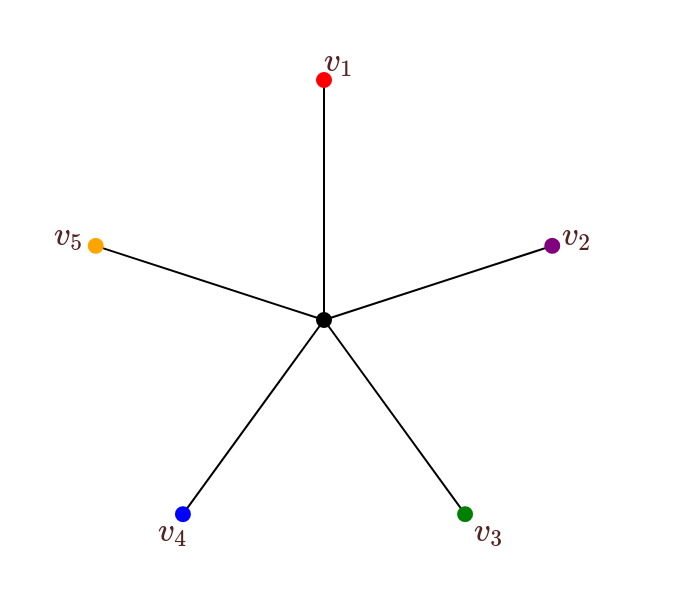
\includegraphics{images/ch5-five-coloring-p1.png}
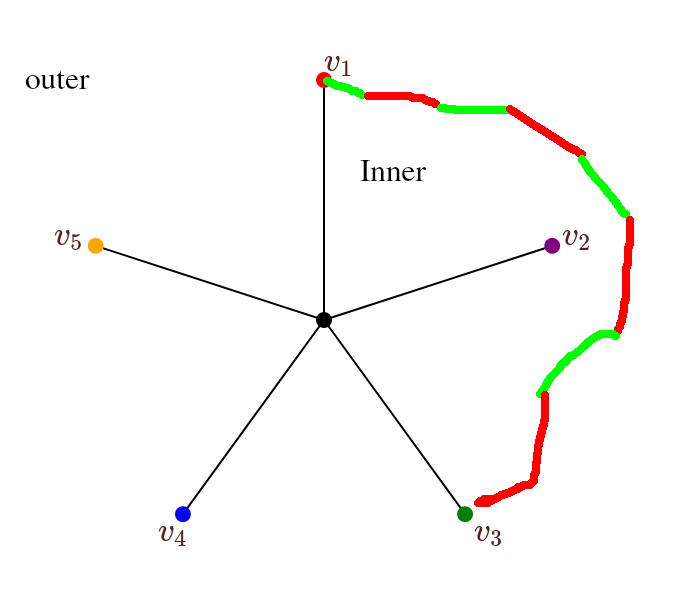
\includegraphics{images/ch5-five-coloring-p2.png}

\newpage

\end{document}
